% Chapter Template

\chapter{Data set} % Main chapter title

\label{Chapter3} % Change X to a consecutive number; for referencing this chapter elsewhere, use \ref{ChapterX}

\lhead{Chapter 3. \emph{Data set}} % Change X to a consecutive number; this is for the header on each page - perhaps a shortened title
The data set we are using has been collected during an another study [3].So, i am describing the method of data collection here of that data.The dataset utilized in this project was tailored from a French research groups work on oculometric changes in MW episodes, Braboszcz and Delorme \cite{grandchamp2014oculometric} and was open to all for EEG analysis under “CeCILL v2.0” license.
%----------------------------------------------------------------------------------------
%	SECTION 1
%----------------------------------------------------------------------------------------

\section{Subjects}
There was two  volunteer participants after providing written informed consent for this experiment.There was two volunteers,one of them was a 25 years old female (say S1)  and another was  a 31 years old male  (say S2) \cite{grandchamp2014oculometric}.Both of them had a normal vision. Both them had  no neurological or mental disorder and both of them are right handed. For their participation,there was no monetary compensation has been provided .The local ethical committee (CPP 2010-A00744-35) had approved  the protocol followed in procedure of data acquisition  \citet{grandchamp2014oculometric}. Both subjects had been practicing meditation and had performed the task before .To accumulate enough data,each subject had to perform 10 sessions, each session was about 20 minutes.The data was collect over course of 5 weeks \cite{grandchamp2014oculometric}.
%-----------------------------------
%	SUBSECTION 1
%-----------------------------------
\section{Procedure}
 
 \begin{figure}
    \centering
    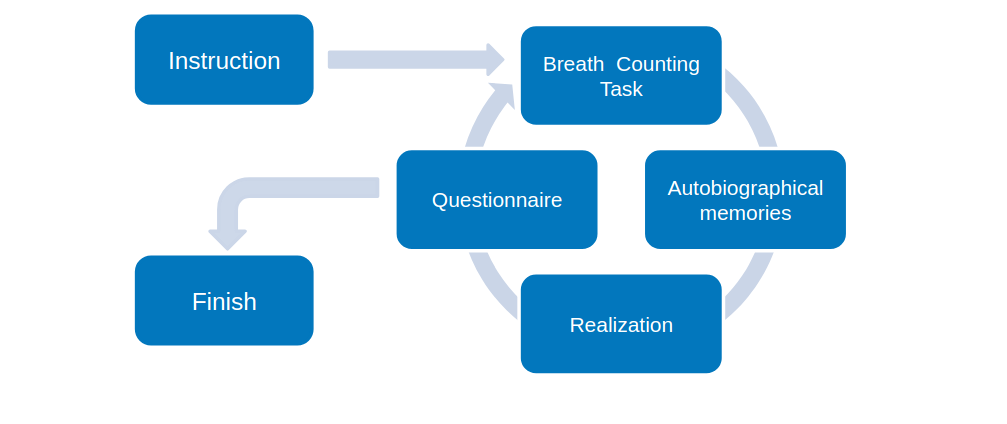
\includegraphics[width=15cm]{Pictures/data_collection.png}
    \caption{data collection flow diagram }
    \label{fig:data_collection}
\end{figure}

The subjects (1 male , 1 female) performed their given task in a dimly lit and soundproof space ahead of a visual display unit .On the display, there were instructions at the beginning of each session.A breath counting task have be performed by the two subjects .They had to count their breath in backward cycles (one inhale and one exhale) from 10 to 1 as one of them reported forward counting even when they were unconscious.By pressing the button,they had reported the realization that they had lost counting of their breath count.After button press, a questionnaire were presented on the screen immediately. It took less than 60 seconds to complete the questionnaire and after the participant's indication process resumed again.A total of 20 session were recorded each of about 20 minute. Using a BioSemi EEG system, EEG signals are recorded from 64 scalp channels from BCI device (an elastic cap) and different biometric channels are concerned in remainder of the channel information recordings. Initial sampling rate of data recording was 1024Hz. Skin Conductance (SC), Electrocardiogram (ECG), further as eye movements and pupil size were additionally recorded. By performing these procedures 19 sessions were recorded of 2 subjects. In this 80 channeled dataset first 64 channels are EEG channels and remainder of the channels are other biometric channels like Pupil size , Gaze position , Skin conductance (SC),Electrocardiogram (ECG) etc. In our paper we only present the findings on EEG information basis .
%  Subjects sat in a dimly lit room with their heads on a chin rest. Instructions were displayed at the beginning of each session on the screen placed at 60 cm in front of them.The task of the subjects was to count backward each of their breath cycles (inhale/exhale) from 10 to 1 \cite{grandchamp2014oculometric}. At 1, they were instructed to restart counting backward from 10.Subjects also had to indicate whenever they realized they had lost track of their breath count (i.e., that their attention had drifted) by pressing the left mouse button.Immediately following the button press, a short 1-page phenomenological questionnaire was presented on the computer screen \cite{grandchamp2014oculometric}. The questionnaire allowed the subject to characterize their mind wandering episodes. After the questionnaire was completed, subjects had to press the right mouse button to indicate they were ready to restart the breath counting task.EEG data were recorded using a 64-channel Bio-semi Active Two system \cite{grandchamp2014oculometric}. Figure ~\ref{fig:data_collection} and Figure ~\ref{fig:single_chanel_data} shows the flow chart of the data collection process.And you can see a sample of collected data in Figure ~\ref{fig:data_sample},blue line indicated by an arrow shows a button click event.


 
 \begin{figure}
    \centering
    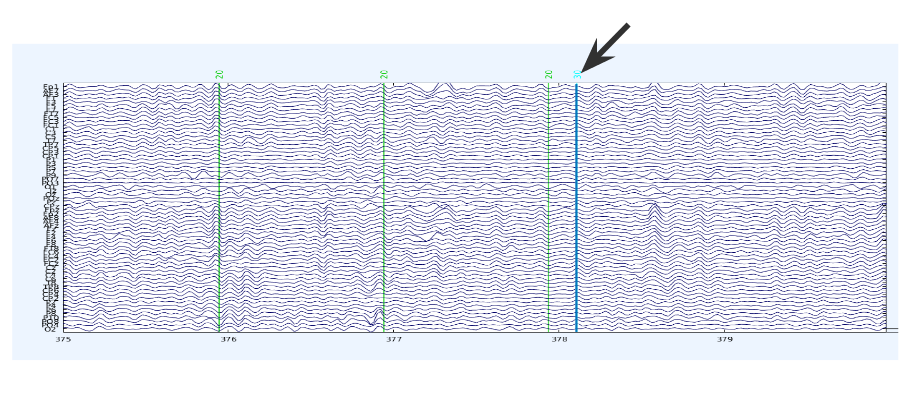
\includegraphics[width=15cm]{Pictures/data_sample.png}
    \caption{A sample of collected data (64 channels) }
    \label{fig:data_sample}
\end{figure}

 \begin{figure}
    \centering
    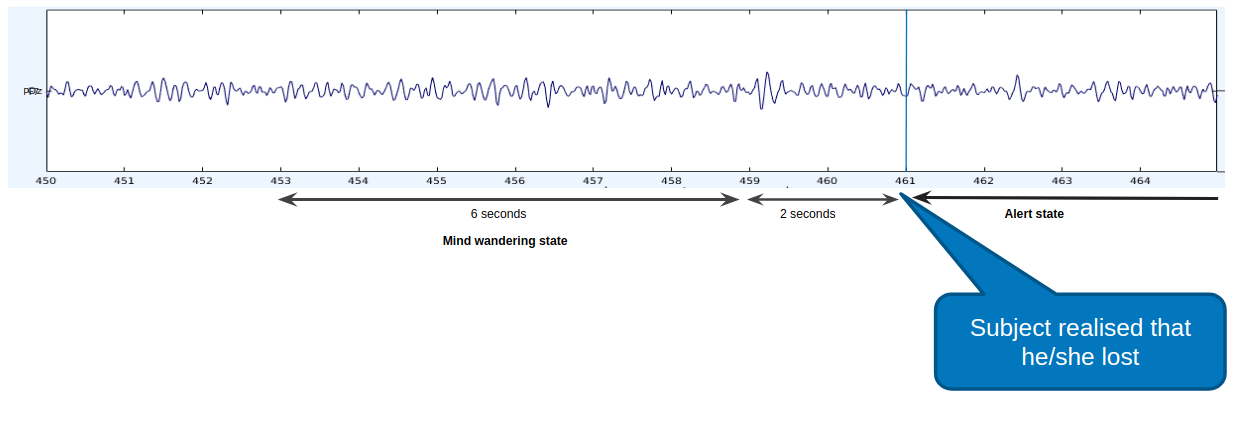
\includegraphics[width=15cm]{Pictures/single_chanel_data.png}
    \caption{Data of a single channel }
    \label{fig:single_chanel_data}
\end{figure}
